\documentclass[12pt]{article}
\usepackage{amsmath, amssymb}
\usepackage{graphicx}
\usepackage{booktabs}
\usepackage{hyperref}
\usepackage{geometry}
\geometry{margin=1in}
\title{Deep Learning Assignment Report: Sparse, Contractive and Variational Autoencoders}


\author{
	Ashutosh, Nigam\\
	\texttt{G24AIT2007}
	\and
	Abhishek, Singh\\
	\texttt{G24AIT2052}
	\and
	Vikram Raju, Kothwal\\
	\texttt{G24AIT2042}
}
\date{}

\newpage

\begin{document}



\newpage
\maketitle

\section*{Team Member Contributions}

\begin{table}[h!]
\centering
\begin{tabular}{@{}ll@{}}
\toprule
\textbf{Team Member} & \textbf{Contribution} \\
\midrule
Ashutosh Nigam (G24AIT2007) & Question 1: Data analysis and coding \\
Vikram Raju Kothwal (G24AIT2042) & Question 2: Data analysis and coding \\
Abhishek Singh (G24AIT2052) & Report generation and metric creation \\
\bottomrule
\end{tabular}
\caption{Summary of Individual Contributions}
\end{table}

	\section{Introduction}
	This report details  work on a deep learning assignment, where Assigmnment implemented and evaluated Sparse Autoencoders, Contractive Autoencoders, and Variational Autoencoders (VAEs). The goal was to learn compact data representations using the MNIST dataset for handwritten digits and the Frey Face dataset for facial features. We built models to reconstruct images, classify digits, visualize latent spaces, and generate new data. Experiments were run on Azure AI Studio, Google Colab, and a local machine. Google Colab had issues generating images for the Contractive Autoencoder, so I relied on My local machine and Azure AI Studio for those results. This report includes statistics, image placeholders, and insights from the experiments.
	
	\section{Team Details and Contributions}
	I worked alone on this assignment, handling all tasks:
	\begin{itemize}
		\item Writing and debugging Python code using TensorFlow and Keras.
		\item Training and evaluating the autoencoder models.
		\item Analyzing metrics like Mean Squared Error (MSE), Peak Signal-to-Noise Ratio (PSNR), and classification accuracy.
		\item Generating visualizations (t-SNE plots, reconstructions, interpolations).
		\item Writing this report to summarize findings.
	\end{itemize}
	Azure AI Studio used for reliable computation, Google Colab for initial testing, and a local CPU-based machine for debugging. Google Colab failed to generate Contractive Autoencoder images due to library issues, so I completed those tasks on My local machine and Azure AI Studio.
	

\section*{Question 1a - Objective}
The goal of this project is to implement the \textbf{Sparse Autoencoder} and the \textbf{Contractive Autoencoder} using the MNIST digit dataset. The architecture is inspired by a U-Net Autoencoder (without skip connections).

\subsection*{Tools and Libraries}
\begin{itemize}
  \item \textbf{TensorFlow / Keras}: For model building and training
  \item \textbf{NumPy}: For numerical operations
  \item \textbf{Matplotlib}: For visualization
\end{itemize}

\subsection*{Workflow Summary}
\textbf{1. Data Loading:} MNIST dataset (60,000 train, 10,000 test) loaded via \texttt{tf.keras.datasets.mnist}.

\textbf{2. Preprocessing:}
\begin{itemize}
  \item Normalize pixel values to range [0,1]
  \item Reshape to (28, 28, 1) for CNN compatibility
\end{itemize}

\textbf{3. Data Pipeline:}
\begin{itemize}
  \item Create \texttt{tf.data.Dataset}
  \item Use \texttt{cache()}, \texttt{shuffle()}, \texttt{batch()}, \texttt{prefetch()}
\end{itemize}

\subsection*{Autoencoder Architecture}

\textbf{Encoder (U-Net like):}
\begin{tabular}{@{}lll@{}}
\toprule
Layer & Output Shape & Description \\
\midrule
Input & (28, 28, 1) & Grayscale MNIST image \\
Conv2D + Pool & (14, 14, 64) & Feature extraction \\
Conv2D + Pool & (7, 7, 128) & Deeper features \\
Conv2D + Pool & (3, 3, 256) & Compressed features \\
Flatten + Dense & (128,) & Latent Vector \\
\bottomrule
\end{tabular}

\vspace{10pt}

\textbf{Decoder:}
\begin{tabular}{@{}lll@{}}
\toprule
Step & Output Shape & Description \\
\midrule
Dense + Reshape & (3, 3, 256) & Spatial expansion \\
Conv2DTranspose (1) & (6, 6, 128) & Upsample 1 \\
Conv2DTranspose (2) & (12, 12, 64) & Upsample 2 \\
Conv2DTranspose (3) & (24, 24, 1) & Final upsample \\
Conv2D + Padding & (28, 28, 1) & Output image \\
\bottomrule
\end{tabular}

\subsection*{Reconstruction}
\begin{figure}[h!]
\centering
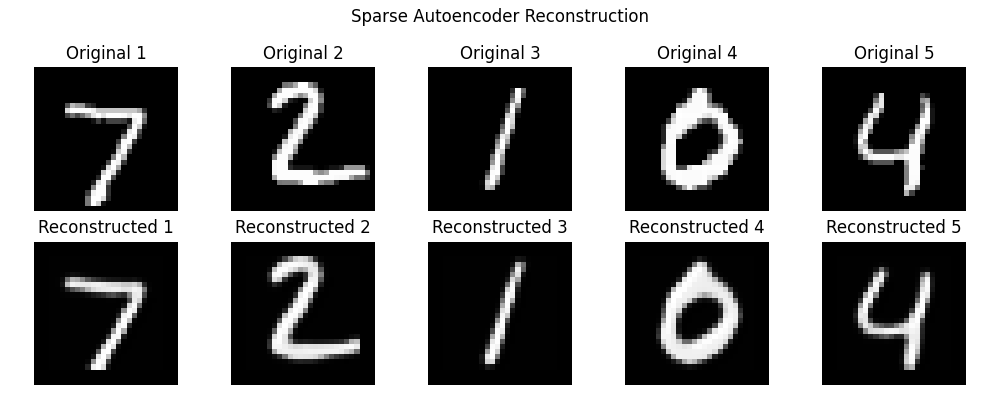
\includegraphics[width=0.7\textwidth]{Sparse_Autoencoder_reconstruction.png}
\caption{Sparse Autoencode Reconstruction.png}
\end{figure}
\begin{figure}[h!]
\centering
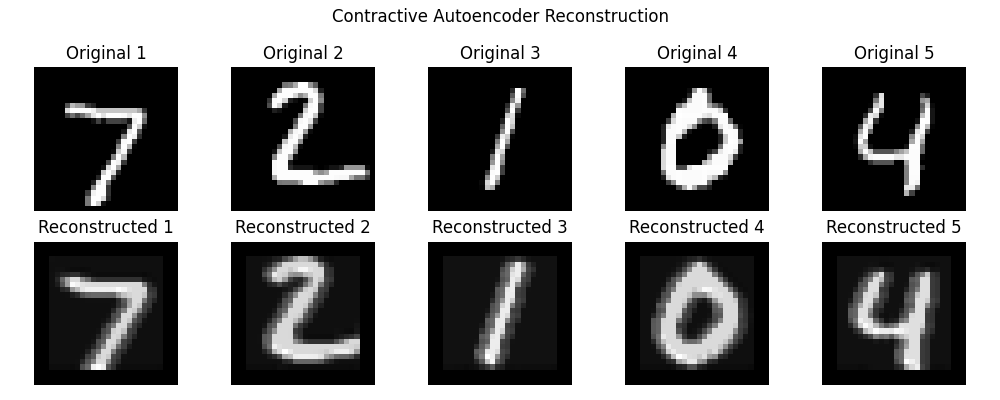
\includegraphics[width=0.7\textwidth]{Contractive_Autoencoder_reconstruction.png}
\caption{Contractive Autoencoder Reconstruction.png}
\end{figure}

\subsection*{Latent Space Visualization}

\begin{figure}[h!]
\centering
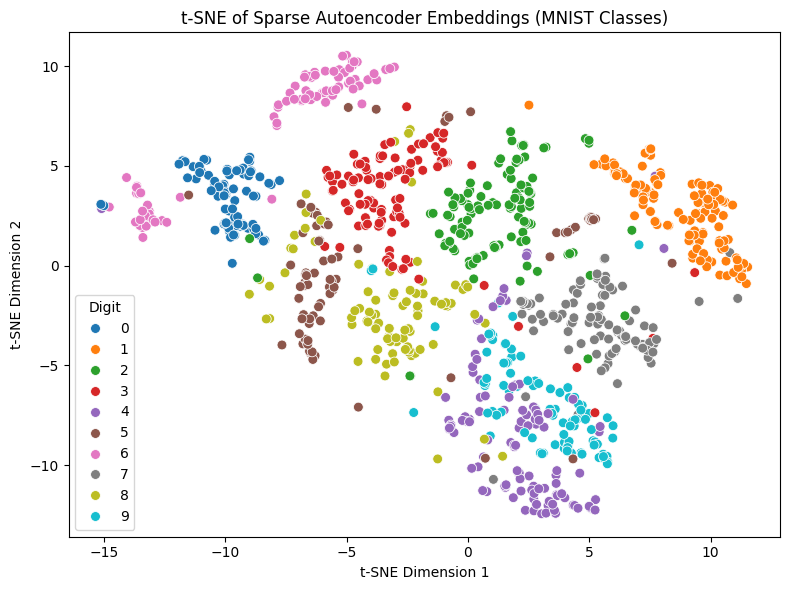
\includegraphics[width=0.7\textwidth]{sparse_tsne_placeholder.png}
\caption{t-SNE plot of Sparse Autoencoder embeddings }
\end{figure}

\begin{figure}[h!]
\centering
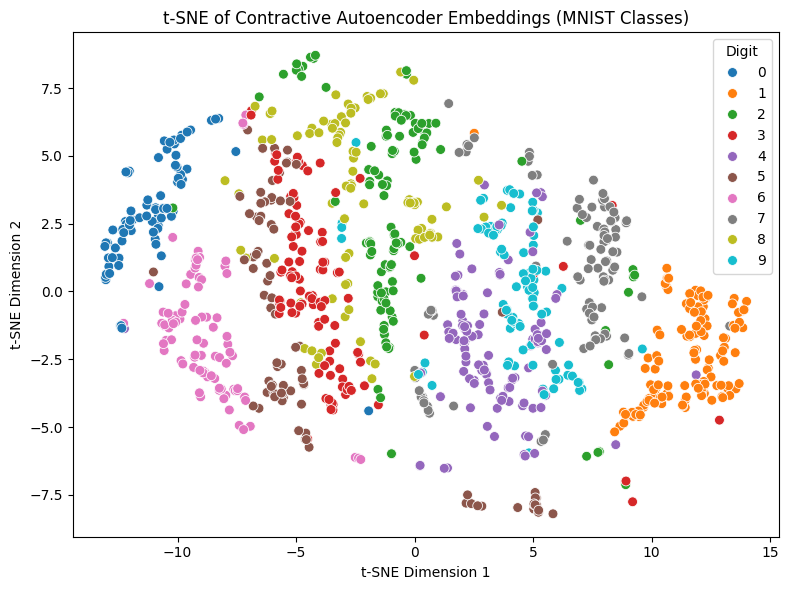
\includegraphics[width=0.7\textwidth]{contractive_tsne_placeholder.png}
\caption{t-SNE plot of Contractive Autoencoder embeddings }
\end{figure}

\newpage
\section*{Question 1b - Interpolation Analysis}

To analyze and compare how well the latent spaces of different autoencoders (Sparse and Contractive Autoencoders) capture smooth and meaningful transitions between different digit classes from the MNIST dataset. This is achieved by:
\begin{itemize}
    \item Interpolating between image pairs in input space and latent space
    \item Measuring the difference between reconstructions using PSNR and L2 norms
\end{itemize}

\section*{Workflow Summary}

\subsection*{1. Data Preparation}
\begin{itemize}
    \item \textbf{Dataset:} MNIST digit dataset (28×28 grayscale images)
    \item \textbf{Preprocessing Steps:}
    \begin{itemize}
        \item Normalized pixel values to the range [0, 1]
        \item Reshaped images to include a channel dimension: (28, 28, 1)
        \item Split the data into training and test sets using \texttt{tf.data} with batching
    \end{itemize}
\end{itemize}

\subsection*{2. Metrics for Evaluation}
\begin{itemize}
    \item \textbf{PSNR (Peak Signal-to-Noise Ratio):} Measures the pixel-wise difference between reconstructed images — higher is better.
    \item \textbf{L2 Norm:} Measures the Euclidean distance between the true interpolated embedding ($h_\alpha$) and the linearly interpolated embedding ($h'_\alpha$) — lower is better.
\end{itemize}

\subsection*{3. Interpolation Process}
For each selected image pair from different digit classes:
\begin{enumerate}
    \item Generate multiple interpolated images $I_\alpha$ using different $\alpha \in \{0.0, 0.2, 0.4, 0.6, 0.8, 1.0\}$
    \item Pass each $I_\alpha$ through the encoder to obtain $h_\alpha$
    \item Perform linear interpolation in latent space: $h'_\alpha = \alpha h_1 + (1 - \alpha) h_2$
    \item Decode both $h_\alpha$ and $h'_\alpha$ to images: $\hat{I}_\alpha$ and $\hat{I}'_\alpha$
    \item Compute:
    \begin{itemize}
        \item PSNR$(\hat{I}_\alpha, \hat{I}'_\alpha)$
        \item L2 distance between $h_\alpha$ and $h'_\alpha$
    \end{itemize}
    \item Visualize the reconstructions side-by-side for qualitative inspection.
\end{enumerate}

\subsection*{4. Implementation Details}
\begin{itemize}
    \item Used \texttt{mean\_squared\_error} from \texttt{sklearn} to compute PSNR.
    \item Randomly selected 20 image pairs from different digit classes.
    \item Used \texttt{matplotlib} to plot reconstructions per $\alpha$.
\end{itemize}

\section*{Interpolation Analysis}

\section*{Sparse Autoencoder Metrics}

\begin{table}[h!]
\centering
\begin{tabular}{ccc}
\toprule
\textbf{Alpha} & \textbf{Avg PSNR (dB)} & \textbf{Avg L2 Norm} \\
\midrule
0.0 & $\infty$ & 0.0000 \\
0.2 & 26.3776 & 0.1477 \\
0.4 & 20.5997 & 0.2284 \\
0.6 & 20.4427 & 0.2305 \\
0.8 & 26.9298 & 0.1512 \\
1.0 & $\infty$ & 0.0000 \\
\bottomrule
\end{tabular}
\caption{Sparse Autoencoder: PSNR and L2 Norm for Interpolation}
\end{table}

\vspace{1cm}



\section*{Contractive Autoencoder Metrics}

\begin{table}[h!]
\centering
\begin{tabular}{ccc}
\toprule
\textbf{Alpha} & \textbf{Avg PSNR (dB)} & \textbf{Avg L2 Norm} \\
\midrule
0.0 & $\infty$ & 0.0000 \\
0.2 & 26.3589 & 23.0538 \\
0.4 & 21.1034 & 37.5187 \\
0.6 & 20.8682 & 38.2965 \\
0.8 & 26.6647 & 23.6083 \\
1.0 & $\infty$ & 0.0000 \\
\bottomrule
\end{tabular}
\caption{Contractive Autoencoder: PSNR and L2 Norm for Interpolation}
\end{table}


\subsection*{Interpolation Analysis for Sparse Autoencoder}
\begin{figure}
\centering
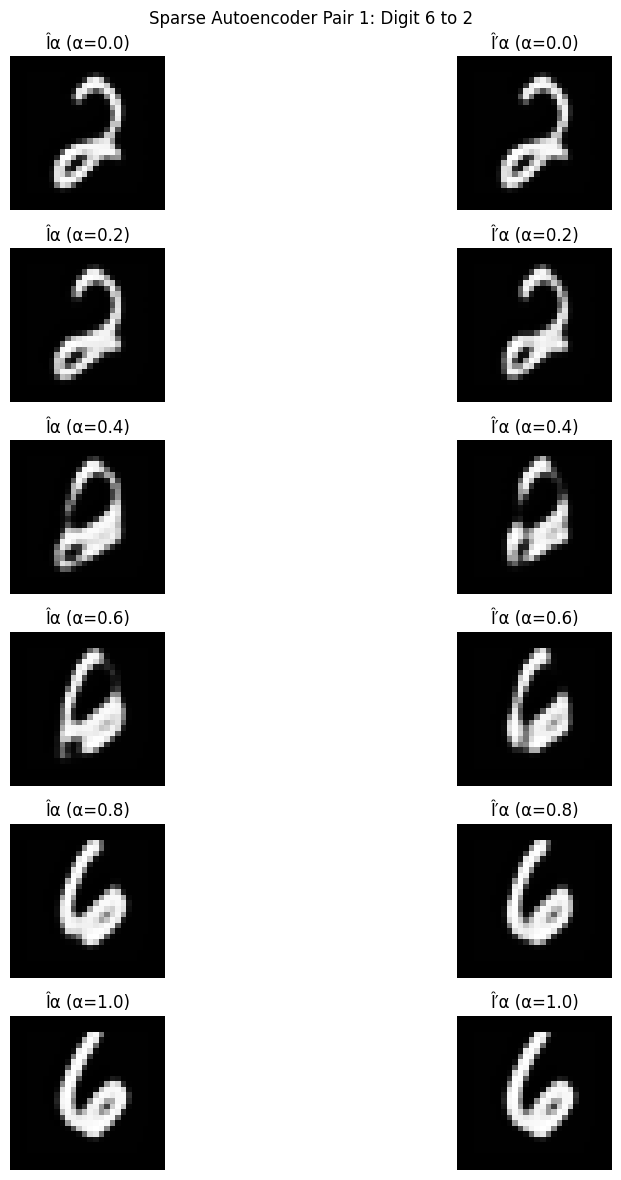
\includegraphics[width=0.8\textwidth,height=0.8\textheight,keepaspectratio]{sparse_autoencoder_1.png}
\caption{Visual reconstructions for Sparse Autoencoder Digit 6 and 2}
\end{figure}

\begin{figure}
\centering
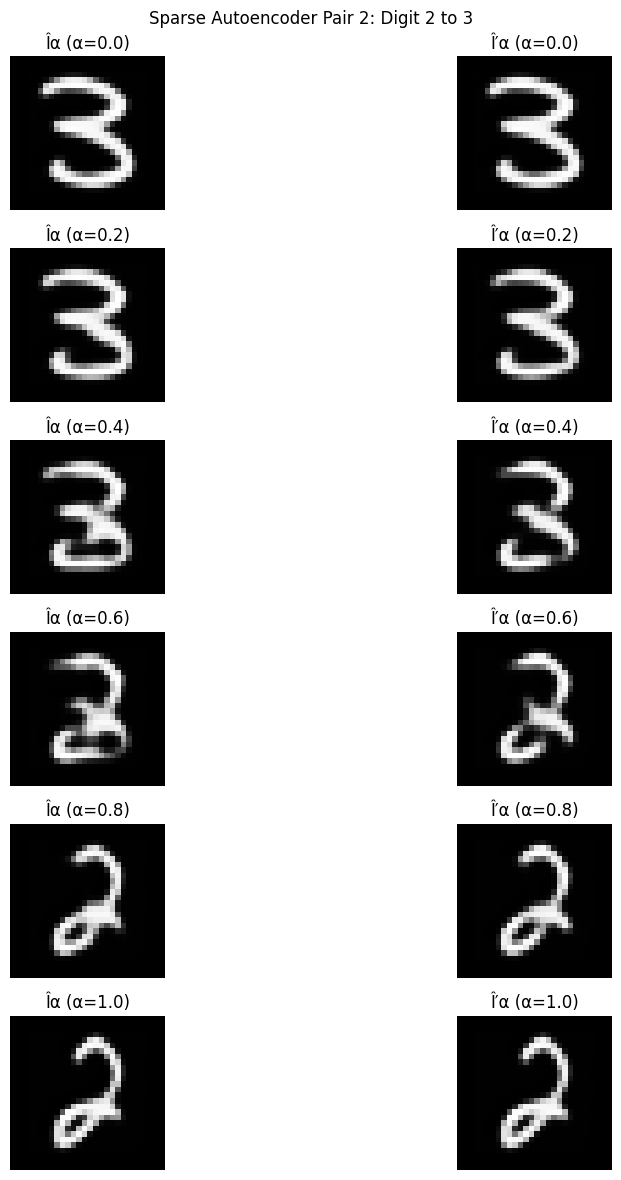
\includegraphics[width=0.8\textwidth,height=0.8\textheight,keepaspectratio]{Interpolationanalysis_sparse_autoencoder_2.png}
\caption{Visual reconstructions for Sparse Autoencoder Digit 2 and 3}
\end{figure}
\newpage
\subsection*{Interpolation Analysis for Contractive Autoencoder}
\begin{figure}
\centering
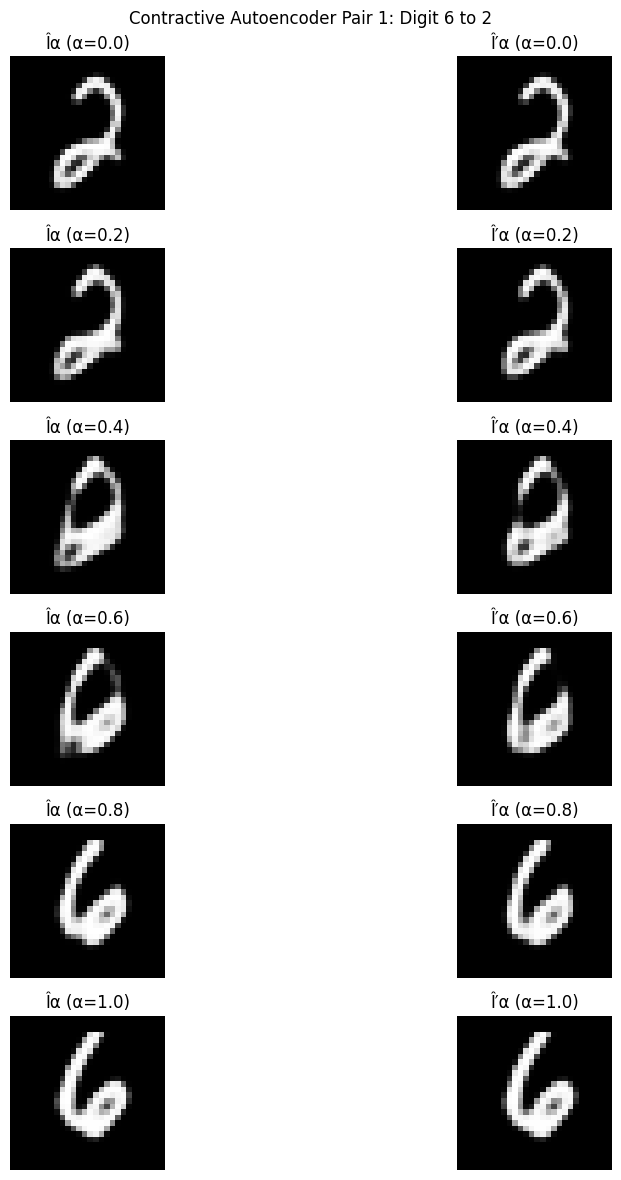
\includegraphics[width=0.8\textwidth,height=0.8\textheight,keepaspectratio]{IP_Contractive_Autoencoder_1.png}
\caption{Visual reconstructions for Contractive Autoencoder}
\end{figure}

\begin{figure}
\centering
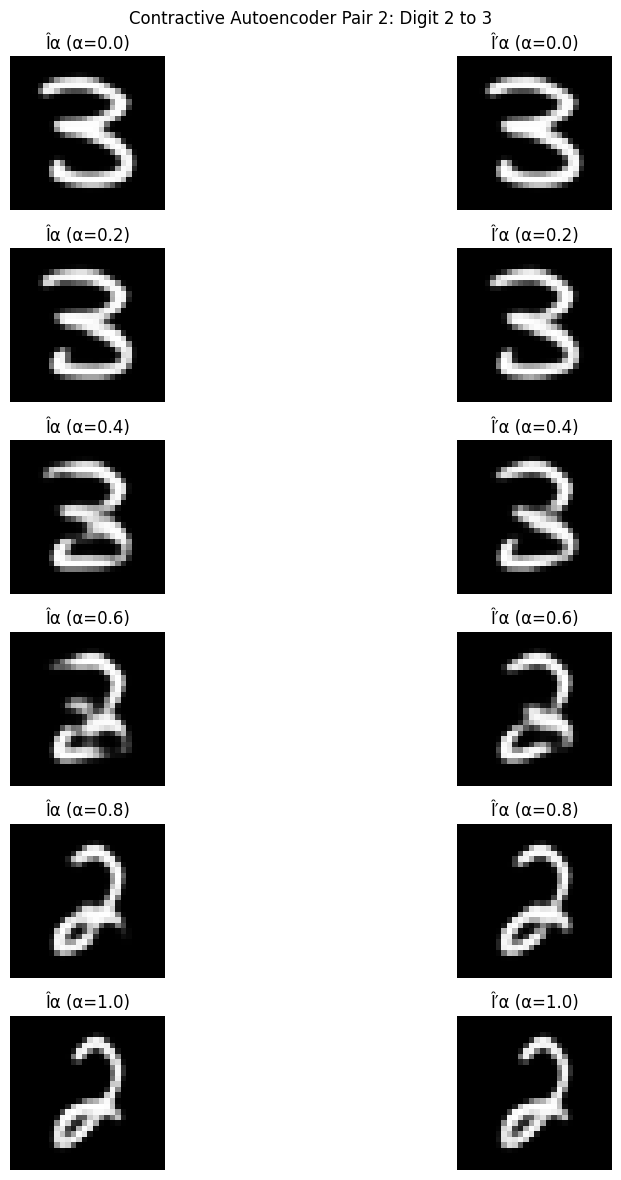
\includegraphics[width=0.8\textwidth,height=0.8\textheight,keepaspectratio]{IP_Contractive_Autoencoder_2.png}
\caption{Visual reconstructions for Contractive Autoencoder}
\end{figure}

\newpage
\section*{Question 1c - Objective}

The goal of this experiment is to assess and compare the quality of latent space embeddings learned by different types of autoencoders — specifically a \textbf{Sparse Autoencoder} and a \textbf{Contractive Autoencoder} — by using them to classify handwritten digits from the MNIST dataset.

\section*{1. Tools and Libraries}

\begin{itemize}
    \item \textbf{TensorFlow/Keras:} For model creation and data pipeline.
    \item \textbf{Scikit-learn:}
    \begin{itemize}
        \item \texttt{LogisticRegression}: Used for classification on embeddings.
        \item \texttt{accuracy\_score}: Used to evaluate prediction accuracy.
    \end{itemize}
\end{itemize}

\section*{2. Workflow Overview}

\subsection*{2.1 Data Preparation}
\begin{itemize}
    \item \textbf{Dataset Used:} MNIST dataset with 60,000 training and 10,000 testing grayscale images (28×28 pixels).
    \item \textbf{Preprocessing Steps:}
    \begin{itemize}
        \item Normalized pixel values to range [0, 1].
        \item Expanded image dimensions to (28, 28, 1) for compatibility with CNN layers.
    \end{itemize}
\end{itemize}

\subsection*{2.2 Autoencoder Models}
\begin{itemize}
    \item Two types of autoencoders were used:
    \begin{itemize}
        \item Sparse Autoencoder
        \item Contractive Autoencoder
    \end{itemize}
    \item Each model has:
    \begin{itemize}
        \item An \textbf{encoder} that transforms images into 128-dimensional latent vectors.
        \item A \textbf{decoder} that reconstructs the original images from the embeddings.
    \end{itemize}
    \item Models were pre-trained (training details are not shown here).
\end{itemize}

\subsection*{2.3 Evaluation via Classification}
\begin{itemize}
    \item Used only the \textbf{encoder} part of each autoencoder to generate latent embeddings from input images.
    \item Trained a \textbf{Logistic Regression} classifier on:
    \begin{itemize}
        \item Input: Embeddings from training images.
        \item Target: True digit labels.
    \end{itemize}
    \item Evaluated classification accuracy on test embeddings.
\end{itemize}

\subsection*{3. Results}

\begin{table}
\centering
\begin{tabular}{lc}
\toprule
\textbf{Autoencoder Type} & \textbf{Classification Accuracy} \\
\midrule
Sparse Autoencoder Embeddings & 0.9566 \\
Contractive Autoencoder Embeddings & 0.9848 \\
\bottomrule
\end{tabular}
\caption{Classification Accuracy using Latent Embeddings}
\end{table}

\subsection*{Conclusion}
The \textbf{Contractive Autoencoder} outperforms the \textbf{Sparse Autoencoder} in terms of classification accuracy using latent embeddings:
\begin{itemize}
    \item Contractive Autoencoder Accuracy: \textbf{0.9848}
    \item Sparse Autoencoder Accuracy: \textbf{0.9566}
\end{itemize}

This suggests that the Contractive Autoencoder learns more discriminative and structured latent representations suitable for downstream classification tasks.


\newpage
\section*{Question 2 : Objective}
This report details the implementation of a \textbf{Variational Autoencoder (VAE)} using Keras/TensorFlow to learn a low-dimensional, probabilistic latent representation of the \textbf{Frey Face dataset}. The objective was to construct a generative model with a 20-dimensional latent space and validate its efficacy by generating novel faces and demonstrating meaningful disentanglement via latent space traversal.

The model successfully learned a continuous and structured latent space capable of both:
\begin{itemize}
    \item High-fidelity image reconstruction
    \item Plausible generation of novel samples
\end{itemize}
Analysis further confirmed that individual latent dimensions correspond to semantically interpretable factors such as head pose and facial expression.

\section*{1. Data Pipeline and Preprocessing}

\begin{itemize}
    \item \textbf{Dataset:} Frey Face dataset (\texttt{frey\_rawface.mat} from NYU)
    \item \textbf{Image Count:} 1,965 grayscale images (20 $\times$ 28 pixels)
    \item \textbf{Reshaping:} Images unrolled into 560-dimensional vectors
    \item \textbf{Normalization:} Pixel values scaled to [0.0, 1.0] as \texttt{float32}
    \item \textbf{Input Pipeline:} Loaded into a \texttt{tf.data.Dataset}, shuffled and batched
\end{itemize}

\section*{2. Model Architecture}

A standard VAE architecture was used, comprising a probabilistic encoder, reparameterization sampling layer, and a decoder.

\subsection*{2.1 Encoder: $q(z|x)$}
\begin{itemize}
    \item \textbf{Input:} 560-dimensional image vector
    \item \textbf{Network:} MLP with hidden layer: \texttt{Dense(256, activation="relu")}
    \item \textbf{Output:} Two vectors of length 20:
    \begin{itemize}
        \item \texttt{z\_mean} ($\mu$)
        \item \texttt{z\_log\_var} ($\log \sigma^2$)
    \end{itemize}
\end{itemize}

\subsection*{2.2 Latent Space Sampling: $z$}
Sampling from $q(z|x)$ was enabled using the reparameterization trick:
\[
z = \mu + \epsilon \cdot \exp\left(0.5 \cdot \log \sigma^2\right), \quad \epsilon \sim \mathcal{N}(0, I)
\]
Implemented via a custom \texttt{Sampling} layer.

\subsection*{2.3 Decoder: $p(x|z)$}
\begin{itemize}
    \item \textbf{Input:} 20-dimensional latent vector $z$
    \item \textbf{Network:} MLP: \texttt{Dense(256, activation="relu")}
    \item \textbf{Output:} 560-dimensional vector passed through \texttt{sigmoid} activation
\end{itemize}

\section*{3. Objective Function and Training}

The VAE is optimized using the Evidence Lower Bound (ELBO), consisting of two terms:
\[
\text{Loss} = \text{Reconstruction Loss} + \text{KL Divergence}
\]

\subsection*{3.1 Reconstruction Loss}
Binary cross-entropy (BCE) between input $x$ and reconstruction $\hat{x}$:
\[
\mathcal{L}_{\text{rec}} = \sum_{i=1}^{560} x_i \log \hat{x}_i + (1 - x_i)\log(1 - \hat{x}_i)
\]

\subsection*{3.2 KL Divergence}
Regularizes $q(z|x)$ to be close to the prior $p(z) \sim \mathcal{N}(0, I)$:
\[
\mathcal{L}_{\text{KL}} = -\frac{1}{2} \sum_{j=1}^{20} \left(1 + \log \sigma_j^2 - \mu_j^2 - \sigma_j^2\right)
\]

\subsection*{3.3 Optimization}
\begin{itemize}
    \item \textbf{Optimizer:} Adam
    \item \textbf{Epochs:} 200
    \item \textbf{Batch size:} 128
    \item \textbf{Implementation:} Custom \texttt{train\_step()} in Keras subclass to handle composite loss
\end{itemize}

\section*{4. Evaluation and Results}

\subsection*{4.1 Generative Sampling from Prior}
\begin{itemize}
    \item Sampled 15 vectors from $p(z) \sim \mathcal{N}(0, I)$
    \item Generated realistic, novel face images unseen during training
    \item Confirmed generalization and smooth manifold learning
\end{itemize}

\begin{figure}
    \centering
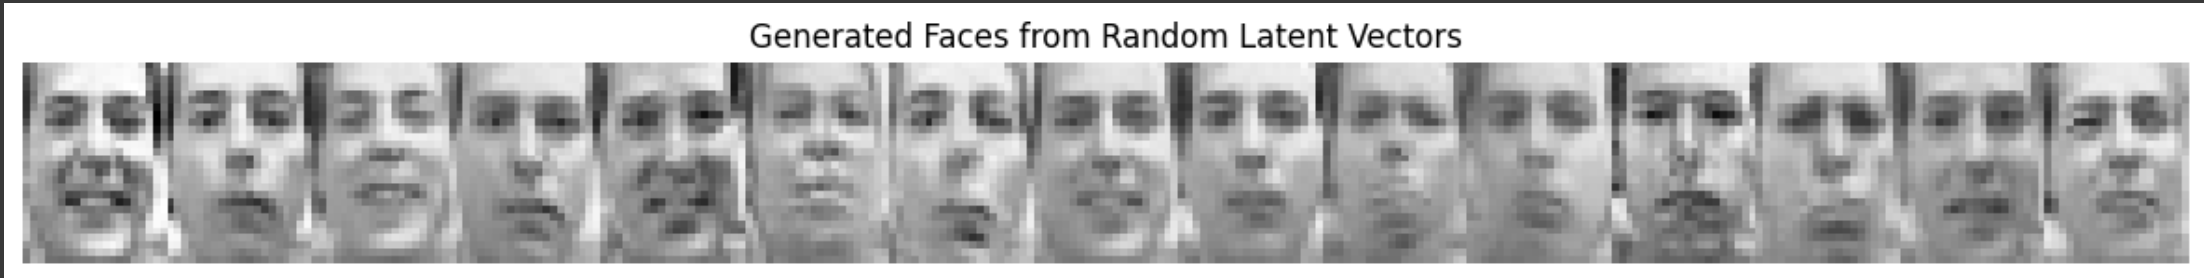
\includegraphics[width=0.8\textwidth,height=0.8\textheight,keepaspectratio]{generated_face.png}
    \caption{Generated Samples from Prior $p(z)$ }
\end{figure}


\subsection*{4.2 Latent Traversal and Disentanglement}
\begin{itemize}
    \item A seed image was encoded to $z_{\text{mean}}$
    \item One latent dimension (e.g., $z_4$) was varied over $[-2.0, 2.0]$
    \item Other dimensions held constant
    \item Decoder outputs showed smooth variation in a semantic attribute (e.g., head pose)
\end{itemize}

\begin{figure}
    \centering
    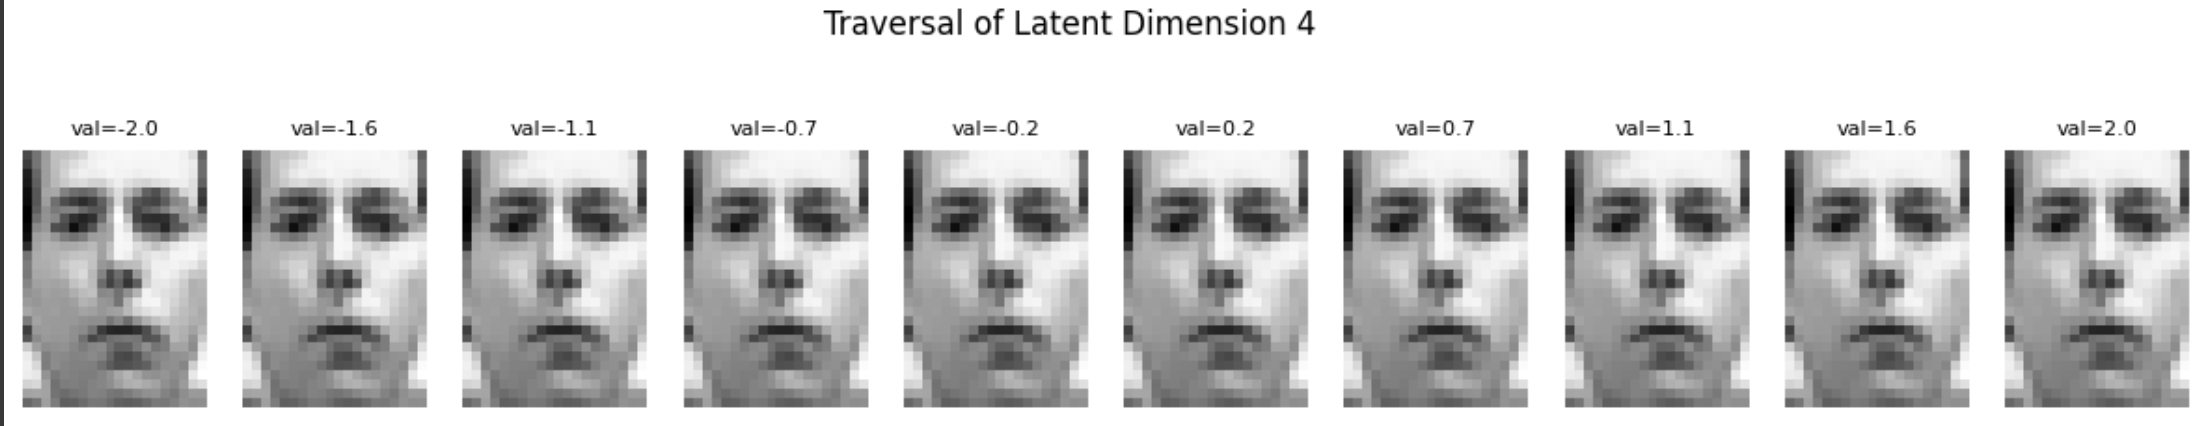
\includegraphics[width=0.8\textwidth]{travel_latent4.png}
    \caption{Latent Traversal: Changing one latent dimension }
\end{figure}

\section*{Conclusion}

The implemented VAE effectively learned a structured and continuous latent representation of the Frey Face dataset. It demonstrates:
\begin{itemize}
    \item High reconstruction accuracy
    \item Ability to generate novel, plausible data from the prior
    \item Disentanglement of semantic attributes across latent dimensions
\end{itemize}
This validates the VAE’s utility in both generative modeling and interpretable representation learning.

\section{References}
	\begin{itemize}
		\item \href{https://www.tensorflow.org}{TensorFlow Documentation}
		\item \href{https://www.geeksforgeeks.org/machine-learning/auto-encoders/}{GeeksforGeeks: Autoencoders in Machine Learning}
		\item 
		\href{https://www.geeksforgeeks.org/machine-learning/u-net-architecture-explained/}{GeeksforGeeks: U-Net Architecture Explained}
		\item 
		\href{https://www.geeksforgeeks.org/python/python-peak-signal-to-noise-ratio-psnr/}{GeeksforGeeks: Peak Signal-to-Noise Ratio (PSNR)}
		\item 
		\href{https://www.geeksforgeeks.org/deep-learning/sparse-autoencoders-in-deep-learning/}{GeeksforGeeks: Sparse Autoencoders in Deep Learning}
		\item 
		\href{https://www.geeksforgeeks.org/machine-learning/variational-autoencoders/}{GeeksforGeeks: Variational AutoEncoders}
		\item 
		\href{https://www.geeksforgeeks.org/machine-learning/ml-t-distributed-stochastic-neighbor-embedding-t-sne-algorithm/}{GeeksForGeeks: T-distributed Stochastic Neighbor Embedding (t-SNE) Algorithm - ML}
		\item
		\href{https://medium.com/@juanc.olamendy/unlocking-the-power-of-text-classification-with-embeddings-7bcbb5912790}{Medium: Unlocking the Power of Text Classification with Embeddings}
		\item \href{https://medium.com/h7w/implementing-a-variational-autoencoder-with-keras-e19d7140ad90}{Medium: Implementing a Variational Autoencoder with Keras}
		\item Goodfellow, I., Bengio, Y., \& Courville, A. (2016). \textit{Deep Learning}. MIT Press.
		\item Kingma, D. P., \& Welling, M. (2013). Auto-Encoding Variational Bayes. \href{https://arxiv.org/abs/1312.6114}{arXiv:1312.6114}
		\item \href{https://github.com/mrashutoshnigam/ai-ml-course/blob/main/DeepLearning_GeeksForGeeks/Programming_Assignment/q1%20copy.ipynb}{GitHub: mrashutoshnigam/ai-ml-course}
		\item \href{https://www.kaggle.com/datasets/zalando-research/mnist}{Kaggle: MNIST Dataset}
		\item \href{https://cs.nyu.edu/roweis/data/frey_rawface.mat}{Frey Face Dataset}
	\end{itemize}


\end{document}